\begin{frame}[plain]
    \hspace{2cm}
    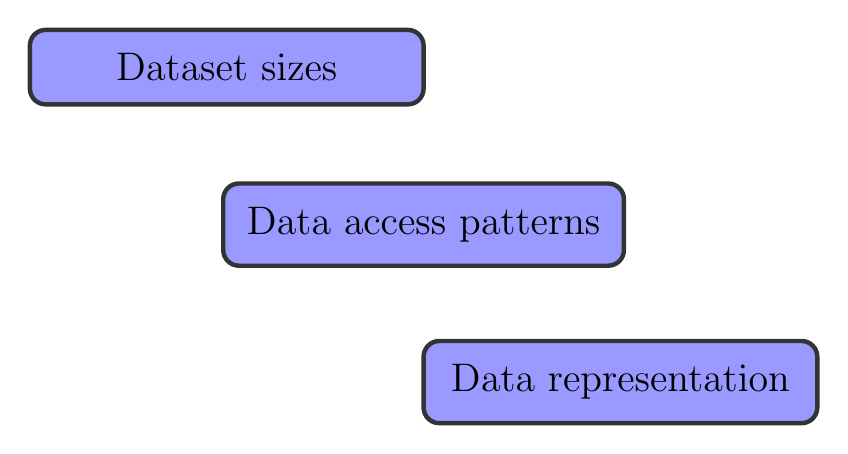
\begin{tikzpicture}[
        norm/.style={draw=black!80,rectangle,rounded corners=2mm,inner sep=3mm,fill=blue!40,ultra thick,minimum width=5cm},
        lit/.style={draw=black!80,rectangle,rounded corners=2mm,inner sep=3mm,fill=red!80,ultra thick,minimum width=5cm}
      ]
      \node[norm] at (0,-0) {{\Large Dataset sizes}};
      \node[norm] at (2.5,-2) {{\Large Data access patterns}};
      \node[norm] at (5,-4) {{\Large Data representation}};
    \end{tikzpicture}
\end{frame}

\begin{frame}[plain]
    \hspace{2cm}
    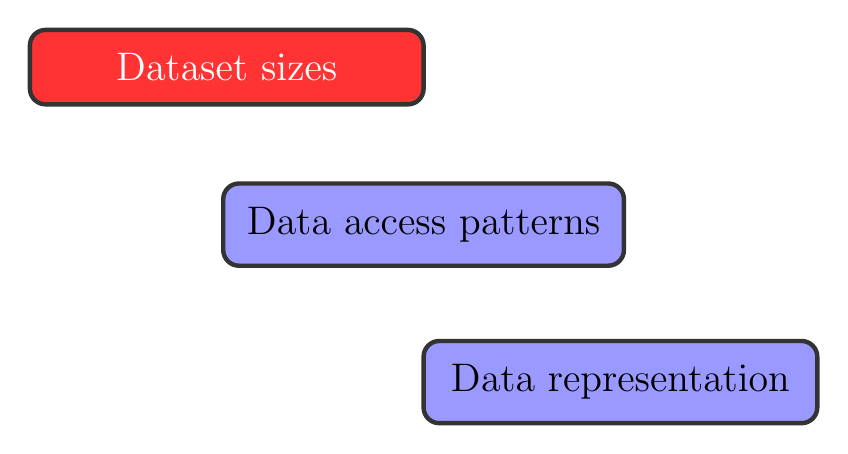
\begin{tikzpicture}[
        norm/.style={draw=black!80,rectangle,rounded corners=2mm,inner sep=3mm,fill=blue!40,ultra thick,minimum width=5cm},
        lit/.style={draw=black!80,rectangle,rounded corners=2mm,inner sep=3mm,fill=red!80,ultra thick,minimum width=5cm}
      ]
      \node[lit] at (0,0) {{\Large \textcolor{white}{Dataset sizes}}};
      \node[norm] at (2.5,-2) {{\Large Data access patterns}};
      \node[norm] at (5,-4) {{\Large Data representation}};
    \end{tikzpicture}
\end{frame}

\begin{frame}[plain]
  \begin{block}{Millennium}
    \begin{itemize}
    \item $\approx$ 750,000,000 galaxies
    \item $\approx$ 300GB
    \item \url{http://www.mpa-garching.mpg.de/galform/virgo/millennium}
    \end{itemize}
  \end{block}
  \begin{block}{Bolshoi}
    \begin{itemize}
    \item $\approx$ 2,500,000,000 galaxies
    \item $\approx$ 1TB
    \item \url{http://hipacc.ucsc.edu/Bolshoi}
    \end{itemize}
  \end{block}
\end{frame}

\begin{frame}[plain]
    \hspace{2cm}
    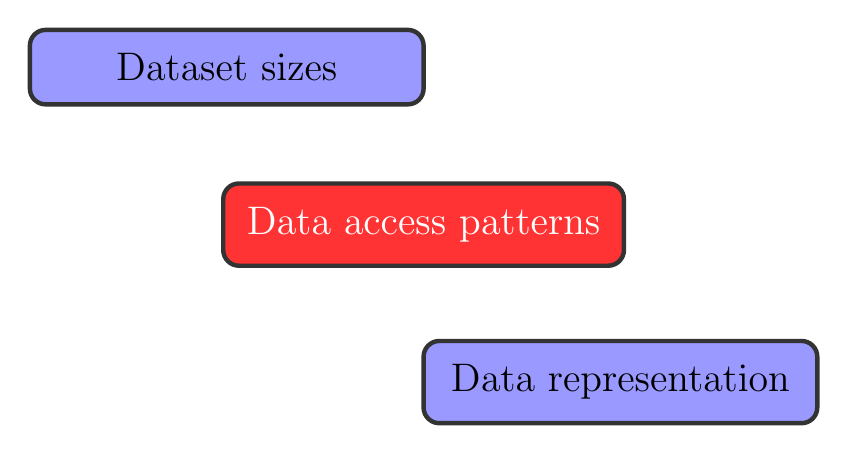
\begin{tikzpicture}[
        norm/.style={draw=black!80,rectangle,rounded corners=2mm,inner sep=3mm,fill=blue!40,ultra thick,minimum width=5cm},
        lit/.style={draw=black!80,rectangle,rounded corners=2mm,inner sep=3mm,fill=red!80,ultra thick,minimum width=5cm}
      ]
      \node[norm] at (0,0) {{\Large Dataset sizes}};
      \node[lit] at (2.5,-2) {{\Large \textcolor{white}{Data access patterns}}};
      \node[norm] at (5,-4) {{\Large Data representation}};
    \end{tikzpicture}
\end{frame}

\begin{frame}[plain]
  \begin{block}{Science Modules}
    \vspace{1cm}
    \hspace{2cm}
    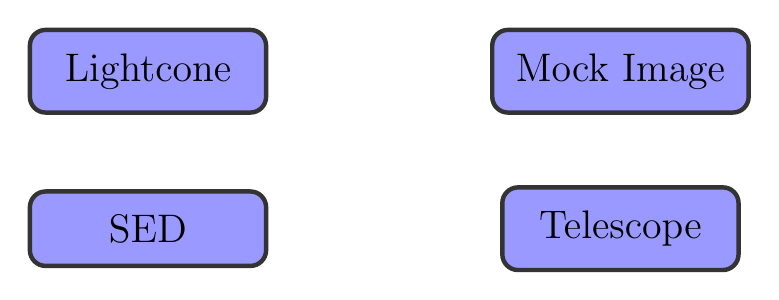
\begin{tikzpicture}[
        norm/.style={draw=black!80,rectangle,rounded corners=2mm,inner sep=3mm,fill=blue!40,ultra thick,minimum width=3cm}
      ]
      \node[norm] at (0,0) {{\Large Lightcone}};
      \node[norm] at (0,-2) {{\Large SED}};
      \node[norm] at (6,0) {{\Large Mock Image}};
      \node[norm] at (6,-2) {{\Large Telescope}};
    \end{tikzpicture}
    \vspace{1cm}
  \end{block}
\end{frame}

\begin{frame}[plain]
  \begin{block}{Science Modules}
    \vspace{1cm}
    \hspace{2cm}
    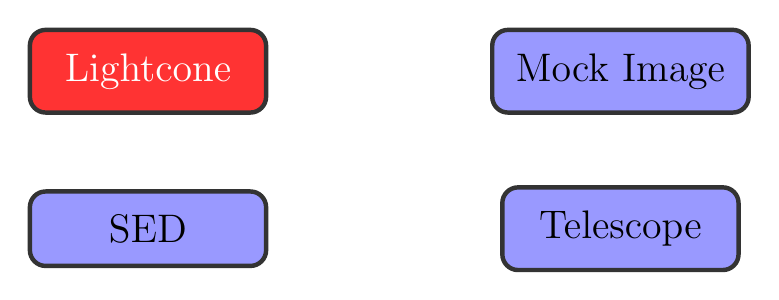
\begin{tikzpicture}[
        norm/.style={draw=black!80,rectangle,rounded corners=2mm,inner sep=3mm,fill=blue!40,ultra thick,minimum width=3cm},
        lit/.style={draw=black!80,rectangle,rounded corners=2mm,inner sep=3mm,fill=red!80,ultra thick,minimum width=3cm}
      ]
      \node[lit] at (0,0) {{\Large \textcolor{white}{Lightcone}}};
      \node[norm] at (0,-2) {{\Large SED}};
      \node[norm] at (6,0) {{\Large Mock Image}};
      \node[norm] at (6,-2) {{\Large Telescope}};
    \end{tikzpicture}
    \vspace{1cm}
  \end{block}
\end{frame}

\begin{frame}[plain]
  \hspace{2cm}
  \begin{tikzpicture}
    \path[use as bounding box] (0,-1) rectangle (10,7);
    % Border.
    \draw (0,0) rectangle(6,6);
    
    \draw[-triangle 90] (8,5.5) node[anchor=west] {simulation domain} -- (6,5);
  \end{tikzpicture}
\end{frame}

\begin{frame}[plain]
  \hspace{2cm}
  \begin{tikzpicture}
    \path[use as bounding box] (0,-1) rectangle (10,7);
    % Border.
    \draw (0,0) rectangle(6,6);
    \draw[-triangle 90] (8,5.5) node[anchor=west] {simulation domain} -- (6,5);
    % Objects.
    \pgfmathsetseed{1187}
    \foreach \x in {1,...,100}
    \fill[black!50] ($ (0,0) + 6*(rnd,rnd) $) circle(1pt);
    \draw[-triangle 90] (8,4.5) node[anchor=west] {galaxies} -- (5,4);
  \end{tikzpicture}
\end{frame}

\begin{frame}[plain]
  \hspace{2cm}
  \begin{tikzpicture}
    \path[use as bounding box] (0,-1) rectangle (10,7);
    % Border.
    \draw (0,0) rectangle(6,6);
    \draw[-triangle 90] (8,5.5) node[anchor=west] {simulation domain} -- (6,5);
    % Objects.
    \pgfmathsetseed{1187}
    \foreach \x in {1,...,100}
    \fill[black!50] ($ (0,0) + 6*(rnd,rnd) $) circle(1pt);
    \draw[-triangle 90] (8,4.5) node[anchor=west] {galaxies} -- (5,4);
    % Cone.
    \filldraw[fill=blue,fill opacity=0.1,draw=blue!90] (0,0) -- (5,3) arc (30.96:59.04:5.83) -- cycle;
    \draw[-triangle 90] (8,3.5) node[anchor=west] {region we want} -- (5,3);
  \end{tikzpicture}
\end{frame}

\begin{frame}[plain]
  \hspace{2cm}
  \begin{tikzpicture}
    \path[use as bounding box] (0,-1) rectangle (10,7);
    % Border.
    \draw (0,0) rectangle(6,6);
    \draw[-triangle 90] (8,5.5) node[anchor=west] {simulation domain} -- (6,5);
    % Objects.
    \pgfmathsetseed{1187}
    \foreach \x in {1,...,100}
    \fill[black!50] ($ (0,0) + 6*(rnd,rnd) $) circle(1pt);
    \draw[-triangle 90] (8,4.5) node[anchor=west] {galaxies} -- (5,4);
    % Cone.
    \filldraw[fill=blue,fill opacity=0.1,draw=blue!90] (0,0) -- (5,3) arc (30.96:59.04:5.83) -- cycle;
    \draw[-triangle 90] (8,3.5) node[anchor=west] {region we want} -- (5,3);
    % Redshift arcs.
    \begin{scope}
      \clip (0,-1) rectangle(6,6);
      \foreach \x/\z in {1.4/0, 2.8/1, 4.2/2, 5.6/3, 7/4}
        \draw[black!75,dashed] (\x,0) node[anchor=north]{$z_\z$} arc (0:90:\x);
    \end{scope}
    \draw[-triangle 90] (8,2.5) node[anchor=west] {time segments} -- (5.6,0.2);
  \end{tikzpicture}
\end{frame}

\begin{frame}[plain]
SELECT * FROM snapshot\_004 WHERE (9437.5 + IF(39.8397 + Pos1 $\langle$ 62.5, 39.8397 + Pos1, Pos1 + 39.8397-62.5) - 0) $\langle$ 9427.7048129608065 AND (9437.5 + IF(39.8397 + Pos1 $\langle$ 62.5, 39.8397 + Pos1, Pos1 + 39.8397-62.5) - 0) $\rangle$ 9408.2000081888491 AND (187.5 + IF(26.503 + Pos2 $\langle$ 62.5, 26.503 + Pos2, Pos2 + 26.503-62.5) - 3.45846e-323) $\langle$ 246.78854155076195 AND (187.5 + IF(26.503 + Pos2 $\langle$ 62.5, 26.503 + Pos2, Pos2 + 26.503-62.5) - 3.45846e-323) $\rangle$ 0 AND (187.5 + IF(55.9087 + Pos3 $\langle$ 62.5, 55.9087 + Pos3, Pos3 + 55.9087-62.5) - 6.90856e-310) $\langle$ 246.78854155076195 AND (187.5 + IF(55.9087 + Pos3 $\langle$ 62.5, 55.9087 + Pos3, Pos3 + 55.9087-62.5) - 6.90856e-310) $\rangle$ 0 AND SQRT(POW((9437.5 + IF(39.8397 + Pos1 $\langle$ 62.5, 39.8397 + Pos1, Pos1 + 39.8397-62.5) - 0), 2)
\end{frame}

\begin{frame}[plain]
+ POW((187.5 + IF(26.503 + Pos2 $\langle$ 62.5, 26.503 + Pos2, Pos2 + 26.503-62.5) - 3.45846e-323), 2) + POW((187.5 + IF(55.9087 + Pos3 $\langle$ 62.5, 55.9087 + Pos3, Pos3 + 55.9087-62.5) - 6.90856e-310), 2)) $\langle$ 9427.7048129608065 AND SQRT(POW((9437.5 + IF(39.8397 + Pos1 $\langle$ 62.5, 39.8397 + Pos1, Pos1 + 39.8397-62.5) - 0), 2) + POW((187.5 + IF(26.503 + Pos2 $\langle$ 62.5, 26.503 + Pos2, Pos2 + 26.503-62.5) - 3.45846e-323), 2) + POW((187.5 + IF(55.9087 + Pos3 $\langle$ 62.5, 55.9087 + Pos3, Pos3 + 55.9087-62.5) - 6.90856e-310), 2)) $\rangle$ 9414.6512343460909 AND SQRT(POW((9437.5 + IF(39.8397 + Pos1 $\langle$ 62.5, 39.8397 + Pos1, Pos1 + 39.8397-62.5) - 0), 2) + POW((187.5 + IF(26.503 + Pos2 $\langle$ 62.5, 26.503 + Pos2, Pos2 + 26.503-62.5) - 3.45846e-323), 2) + POW((187.5 + IF(55.9087 + Pos3 $\langle$ 62.5, 55.9087 + Pos3, Pos3 + 55.9087-62.5) - 6.90856e-310), 2)) $\langle$ 9427.7048129608065 AND
\end{frame}

\begin{frame}[plain]
(9437.5 + IF(39.8397 + Pos1 $\langle$ 62.5, 39.8397 + Pos1, Pos1 + 39.8397 - 62.5) - 0)/(SQRT(POW((9437.5 + IF(39.8397 + Pos1 $\langle$ 62.5, 39.8397 + Pos1, Pos1 + 39.8397 - 62.5) - 0), 2) + POW((187.5 + IF(26.503 + Pos2 $\langle$ 62.5, 26.503 + Pos2, Pos2 + 26.503 - 62.5) - 3.45846e-323), 2))) $\rangle$ 0.070737201667702906 AND (9437.5 + IF(39.8397 + Pos1 $\langle$ 62.5, 39.8397 + Pos1, Pos1 + 39.8397 - 62.5) - 0)/(SQRT(POW((9437.5 + IF(39.8397 + Pos1 $\langle$ 62.5, 39.8397 + Pos1, Pos1 + 39.8397 - 62.5) - 0), 2) + POW((187.5 + IF(26.503 + Pos2 $\langle$ 62.5, 26.503 + Pos2, Pos2 + 26.503-62.5) - 3.45846e-323), 2))) $\langle$ 1 AND SQRT(POW((9437.5 + IF(39.8397 + Pos1 $\langle$ 62.5, 39.8397 + Pos1, Pos1 + 39.8397-62.5) - 0), 2) + POW((187.5 + IF(26.503 + Pos2 $\langle$ 62.5, 26.503 + Pos2, Pos2 + 26.503-62.5) -
\end{frame}

\begin{frame}[plain]
3.45846e-323), 2))/(SQRT(POW((9437.5 + IF(39.8397 + Pos1 $\langle$ 62.5, 39.8397 + Pos1, Pos1 + 39.8397-62.5) - 0), 2) + POW((187.5 + IF(26.503 + Pos2 $\langle$ 62.5, 26.503 + Pos2, Pos2 + 26.503-62.5) - 3.45846e-323), 2) + POW((187.5 + IF(55.9087 + Pos3 $\langle$ 62.5, 55.9087 + Pos3, Pos3 + 55.9087-62.5) - 6.90856e-310), 2))) $\rangle$ 0.070737201667702906 AND SQRT(POW((9437.5 + IF(39.8397 + Pos1 $\langle$ 62.5, 39.8397 + Pos1, Pos1 + 39.8397-62.5) - 0), 2) + POW((187.5 + IF(26.503 + Pos2 $\langle$ 62.5, 26.503 + Pos2, Pos2 + 26.503-62.5) - 3.45846e-323), 2))/(SQRT(POW((9437.5 + IF(39.8397 + Pos1 $\langle$ 62.5, 39.8397 + Pos1, Pos1 + 39.8397-62.5) - 0), 2) + POW((187.5 + IF(26.503 + Pos2 $\langle$ 62.5, 26.503 + Pos2, Pos2 + 26.503-62.5) - 3.45846e-323), 2) + POW((187.5 + IF(55.9087 + Pos3 $\langle$ 62.5, 55.9087 + Pos3, Pos3 + 55.9087-62.5) - 6.90856e-310), 2))) $\langle$ 1
\end{frame}

\begin{frame}[plain]
  \hspace{2.5cm}{\Large Very large amount of data to search} \\
  \hspace{2cm}{\Large + Complicated SQL query} \\
  \hspace{2cm}{\Large + Multiple users} \\
  \hspace{2cm}{\Large = \alert{Trouble}}
  \vspace{1cm}
  \begin{alertblock}{Solution}
    \centering
    \vspace{0.5cm}
    {\Large Distribute over multiple servers.}
    \vspace{0.5cm}
  \end{alertblock}
\end{frame}

\begin{frame}[plain]
 \begin{block}{Distributed DBMS Systems}
 \begin{itemize}
   \item MySQL Cluster
     \begin{itemize}
       \item Difficult to manage.
     \end{itemize}
   \item pgpool
     \begin{itemize}
       \item Bugs with some queries.
     \end{itemize}
   \item PostgresXC
     \begin{itemize}
       \item Older PostgresQL.
       \item Small development team.
     \end{itemize}
   \item Custom (PostgresQL)
     \begin{itemize}
       \item Reinventing the wheel?
     \end{itemize}
 \end{itemize}
 \end{block}
\end{frame}

\begin{frame}[plain]
  \vspace{1cm}
  \begin{center}
 \begin{tikzpicture}
   % Text.
   \node at (-3,3) {We can do better!};
   % Border.
   \draw (0,0) rectangle(6,6);
   % Objects.
   \pgfmathsetseed{1187}
   \foreach \x in {1,...,100}
     \fill[black!50] ($ (0,0) + 6*(rnd,rnd) $) circle(1pt);
   % Cone.
   \filldraw[fill=blue,fill opacity=0.1,draw=blue!90] (0,0) -- (5,3) arc (30.96:59.04:5.83) -- cycle;
    % Redshift arcs.
    \begin{scope}
      \clip (0,-1) rectangle(6,6);
      \foreach \x/\z in {1.4/0, 2.8/1, 4.2/2, 5.6/3, 7/4}
        \draw[black!75,dashed] (\x,0) node[anchor=north]{$z_\z$} arc (0:90:\x);
    \end{scope}
 \end{tikzpicture}
 \end{center}
\end{frame}

\begin{frame}[plain]
  \vspace{1cm}
  \begin{center}
 \begin{tikzpicture}
   % Text.
   \node at (-3,3) {We can do better!};
   % Border.
   \clip (0,-1) rectangle(6,6);
   \draw (0,0) rectangle(6,6);
   % Objects.
   \pgfmathsetseed{1187}
   \foreach \x in {1,...,100}
     \fill[black!50] ($ (0,0) + 6*(rnd,rnd) $) circle(1pt);
   % Cone.
   \filldraw[fill=blue,fill opacity=0.1,draw=blue!90] (0,0) -- (5,3) arc (30.96:59.04:5.83) -- cycle;
    % Redshift arcs.
    \begin{scope}
      \clip (0,-1) rectangle(6,6);
      \foreach \x/\z in {1.4/0, 2.8/1, 4.2/2, 5.6/3, 7/4}
        \draw[black!75,dashed] (\x,0) node[anchor=north]{$z_\z$} arc (0:90:\x);
    \end{scope}
   % Tree cells.
   \draw[step=1.5] (0,0) grid (6,6);
   \draw (2.25,3) -- (2.25,4.5); \draw (1.5,3.75) -- (3,3.75);
   \draw (5.25,1.5) -- (5.25,3); \draw (4.5,2.25) -- (6,2.25);
   \draw (3.75,4.5) -- (3.75,6); \draw (3,5.25) -- (4.5,5.25);
 \end{tikzpicture}
 \end{center}
\end{frame}

\begin{frame}[plain]
  \vspace{1cm}
  \begin{center}
 \begin{tikzpicture}
   % Text.
   \node at (-3,3) {We can do better!};
   % Border.
   \clip (0,-1) rectangle(6,6);
   \draw (0,0) rectangle(6,6);
   % Objects.
   \pgfmathsetseed{1187}
   \foreach \x in {1,...,100}
     \fill[black!50] ($ (0,0) + 6*(rnd,rnd) $) circle(1pt);
   % Cone.
   \filldraw[fill=blue,fill opacity=0.1,draw=blue!90] (0,0) -- (5,3) arc (30.96:59.04:5.83) -- cycle;
    % Redshift arcs.
    \begin{scope}
      \clip (0,-1) rectangle(6,6);
      \foreach \x/\z in {1.4/0, 2.8/1, 4.2/2, 5.6/3, 7/4}
        \draw[black!75,dashed] (\x,0) node[anchor=north]{$z_\z$} arc (0:90:\x);
    \end{scope}
   % Tree cells.
   \fill[fill=red,opacity=0.5] (3,0) rectangle (4.5,1.5);
   \fill[fill=red,opacity=0.5] (4.5,0) rectangle (6,1.5);
   \fill[fill=red,opacity=0.5] (0,3) rectangle (1.5,4.5);
   \fill[fill=red,opacity=0.5] (0,4.5) rectangle (1.5,6);
   \fill[fill=red,opacity=0.5] (4.5,4.5) rectangle (6,6);
   \fill[fill=red,opacity=0.5] (4.5,1.5) rectangle (5.25,2.25);
   \fill[fill=red,opacity=0.5] (5.25,1.5) rectangle (6,2.25);
   \fill[fill=red,opacity=0.5] (5.25,2.25) rectangle (6,3);
   \fill[fill=red,opacity=0.5] (3,5.25) rectangle (4.5,6);
   %% \fill[fill=red,opacity=0.5] (3.75,4.5) rectangle (4.5,5.25);
   \draw[step=1.5] (0,0) grid (6,6);
   \draw (2.25,3) -- (2.25,4.5); \draw (1.5,3.75) -- (3,3.75);
   \draw (5.25,1.5) -- (5.25,3); \draw (4.5,2.25) -- (6,2.25);
   \draw (3.75,4.5) -- (3.75,6); \draw (3,5.25) -- (4.5,5.25);
 \end{tikzpicture}
  \end{center}
\end{frame}
